\section{Versuchsaufbau und Durchführung}
\label{sec:Durchführung}

%unterschiedliche Hallsonden longitudinal und transversal???? die in kurze/lange spule ist longitudinal
\begin{figure}[h!]
        \centering
        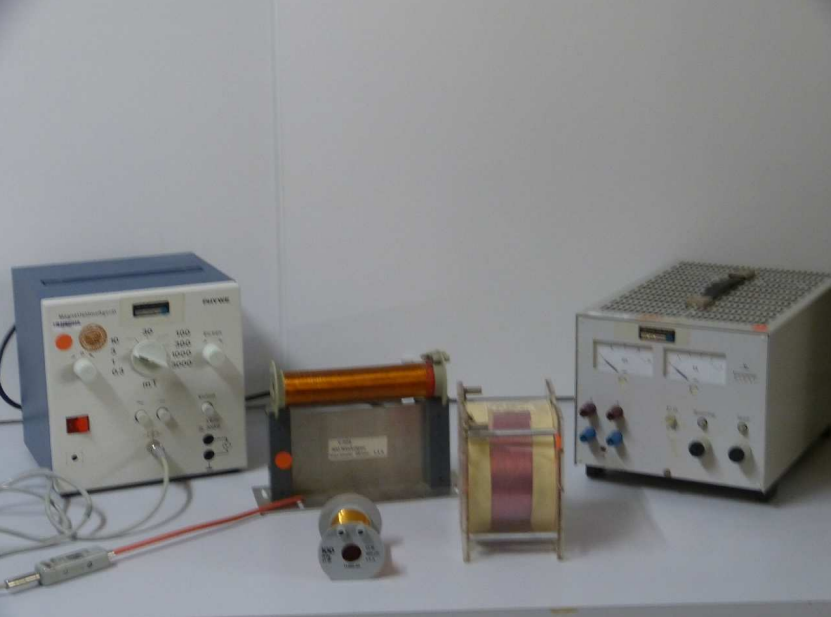
\includegraphics[width=0.3\linewidth]{fotos/spulen.png}
        \caption{Spulen für den ersten Teil des Versuches.\cite{V308}}
        \label{fig:spulen}
\end{figure}
Der Versuch ist in drei Teile aufgeteilt. In allen Aufgabenteilen werden Hallsonden zum messen der magnetischen Flußdichte verwendet.
Für den ersten Teil werden eine lange und eine kurze Spule benötigt. Eine longitudinale Hallsonde wird in die jeweilige Spule geschoben 
und in kleinen Abständen wird die magnetische Flußdichte gemessen.
\\
\begin{figure}[h!]
    \centering
    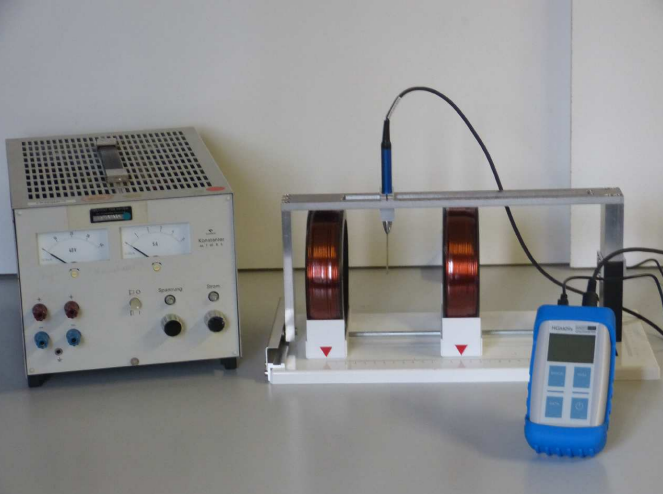
\includegraphics[width=0.3\linewidth]{fotos/helmholtz.png}
    \caption{Spulenpaar mit variablem Abstand.\cite{V308}}
    \label{fig:helmholtz}
\end{figure}
\\
Im zweiten Teil des Versuches werden die magnetische Flußdichten eines Spulenpaares gemessen. Eine der beiden Spulen befindet sich auf Schienen 
und kann auf diesen verschoben werden. An der oberen Schiene ist eine transversale Hallsonde befestigt, mit der die Flußdichte an beliebigen 
Stellen zwischen oder außerhalb der Spulen gemessen werden kann. Für alle drei Spulenkonfigurationen werden mehrere Messwerte aufgenommen.
\\
\begin{figure}
    \centering
    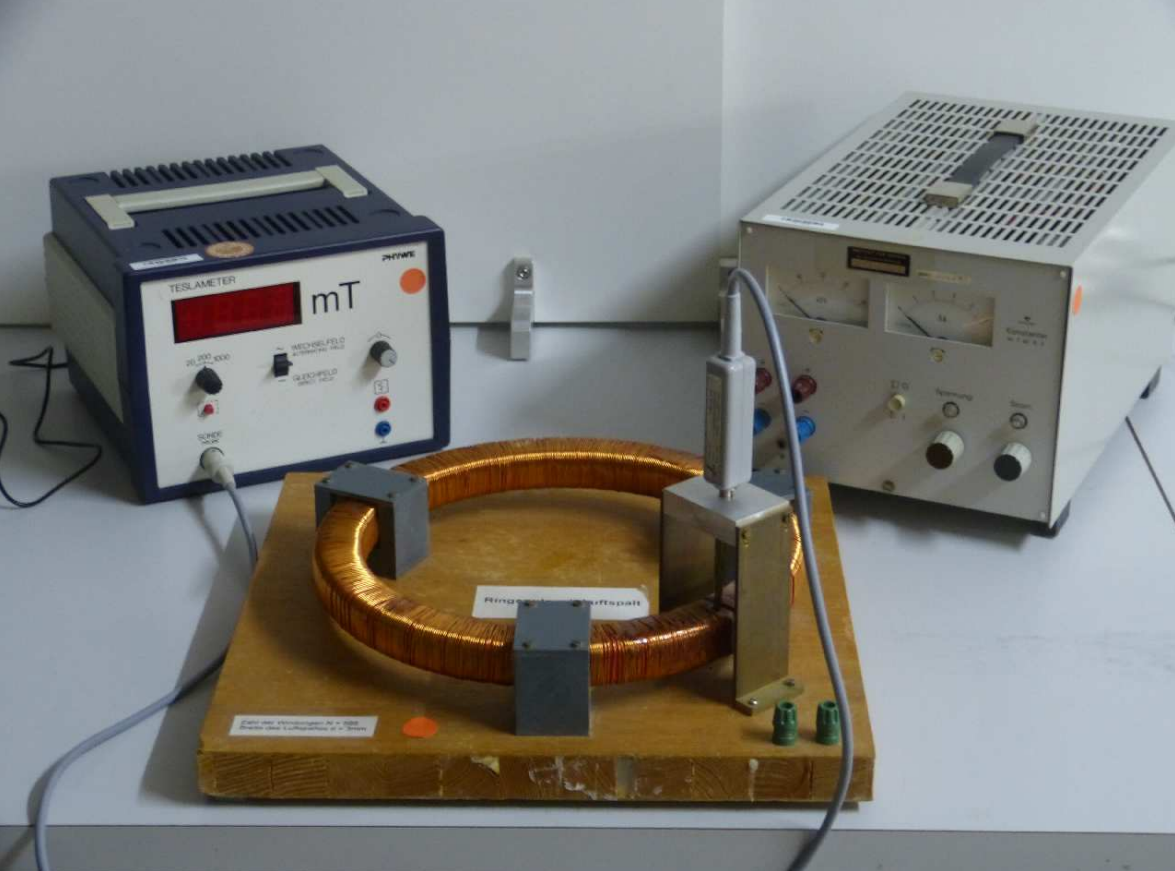
\includegraphics[width=0.3\linewidth]{fotos/hysterese.png}
    \caption{Teslameter und Ringspule mit Luftspalt.\cite{V308}}
    \label{fig:ringspule}
\end{figure}
Im dritten Teil des Versuches wird eine Hysteresekurve einer Ringspule mit Luftspalt aufgenommen. Die Spule besitzt einen ferromagnetischen Kern.
Zu erst wird der Kern mit einer angelegten Wechselspannung entmagnetisiert. Dann wird mit einem Spannungsgerät bei voll aufgedrehtem Spannungsregler in Schritten von 
$\SI{0.5}{\ampere}$ der Stromfluss erhöht. Mit einem Teslameter wird die Flußdichte ermittelt.
\newpage